\documentclass{article}
\usepackage[utf8]{inputenc}
\usepackage{listings}
\usepackage[french]{babel}
\usepackage{graphicx}
\usepackage{pifont}
\usepackage[left=2.5cm,right=2.5cm,top=3cm,bottom=3cm]{geometry}
\renewcommand{\baselinestretch}{1.3}
\lstset{
  basicstyle=\small,
  mathescape
}
\lstset{literate=
  {á}{{\'a}}1 {é}{{\'e}}1 {í}{{\'i}}1 {ó}{{\'o}}1 {ú}{{\'u}}1
  {Á}{{\'A}}1 {É}{{\'E}}1 {Í}{{\'I}}1 {Ó}{{\'O}}1 {Ú}{{\'U}}1
  {à}{{\`a}}1 {è}{{\`e}}1 {ì}{{\`i}}1 {ò}{{\`o}}1 {ù}{{\`u}}1
  {À}{{\`A}}1 {È}{{\'E}}1 {Ì}{{\`I}}1 {Ò}{{\`O}}1 {Ù}{{\`U}}1
  {ä}{{\"a}}1 {ë}{{\"e}}1 {ï}{{\"i}}1 {ö}{{\"o}}1 {ü}{{\"u}}1
  {Ä}{{\"A}}1 {Ë}{{\"E}}1 {Ï}{{\"I}}1 {Ö}{{\"O}}1 {Ü}{{\"U}}1
  {â}{{\^a}}1 {ê}{{\^e}}1 {î}{{\^i}}1 {ô}{{\^o}}1 {û}{{\^u}}1
  {Â}{{\^A}}1 {Ê}{{\^E}}1 {Î}{{\^I}}1 {Ô}{{\^O}}1 {Û}{{\^U}}1
  {œ}{{\oe}}1 {Œ}{{\OE}}1 {æ}{{\ae}}1 {Æ}{{\AE}}1 {ß}{{\ss}}1
  {ű}{{\H{u}}}1 {Ű}{{\H{U}}}1 {ő}{{\H{o}}}1 {Ő}{{\H{O}}}1
  {ç}{{\c c}}1 {Ç}{{\c C}}1 {ø}{{\o}}1 {å}{{\r a}}1 {Å}{{\r A}}1
  {€}{{\euro}}1 {£}{{\pounds}}1 {«}{{\guillemotleft}}1
  {»}{{\guillemotright}}1 {ñ}{{\~n}}1 {Ñ}{{\~N}}1 {¿}{{?`}}1
}
\author{Alexis Lanoix et Jofrey Luc}
\title{Rapport init recherche}
\date{02/05/2017}

\begin{document}

\tableofcontents
\newpage

\section{Introduction et problématique}

Aujourd'hui, on dispose de moyens assez efficaces pour transformer automatiquement un texte prononcé dans un fichier audio en sa transcription écrite (par exemple, l'outil de sous-titrage automatique de Youtube). Le problème avec ces outils est qu'ils nécessitent toujours de savoir en quelle langue le texte est prononcé pour pouvoir le transcrire efficacement.\\
En effet, pour faire de la reconnaissance de la parole, il est essentiel de connaître le langage à traduire au préalable car il faut pouvoir utiliser les éléments propres à celui-ci.\\

\begin{figure}[h]
  \centerline{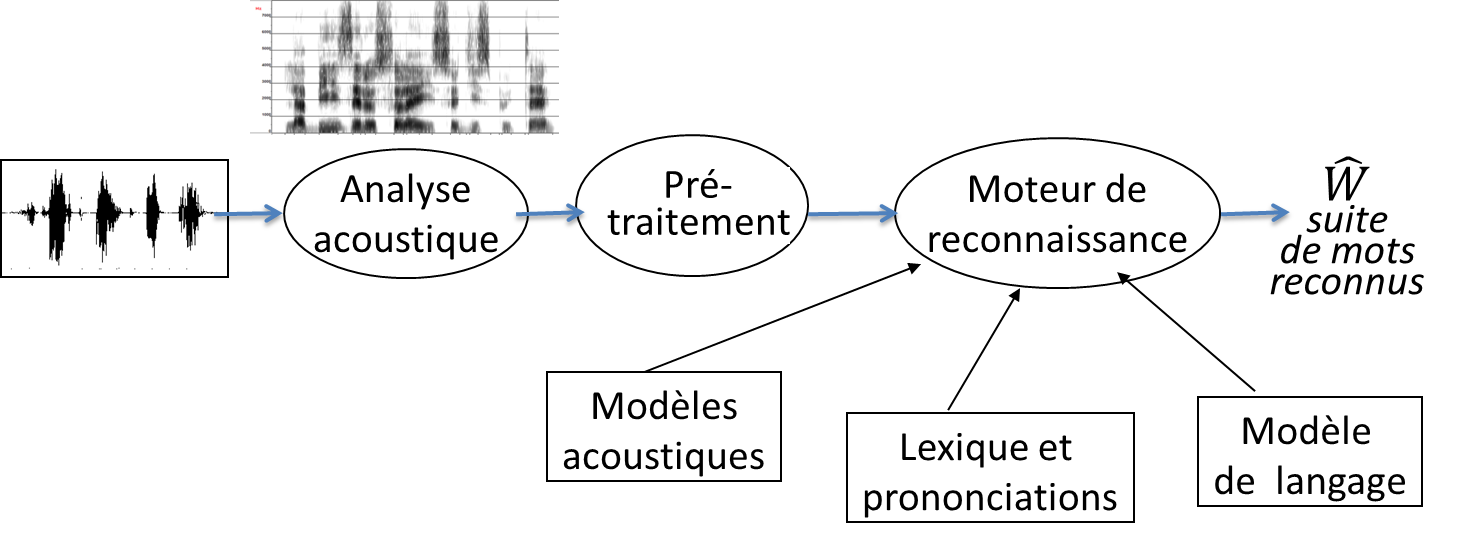
\includegraphics[scale=0.6]{img/schema_reco.png}}
  \caption{Schéma d'un système classique de reconnaissance de la parole}
\end{figure}

\noindent Ici, les éléments qui vont changer d'un langage à l'autre sont les modèles acoustiques, le lexique et les prononciations et le modèle de langage.\\
 \\
L'objectif de ce projet d'initiation à la recherche est donc de parvenir à détecter automatiquement la langue parlée dans un fichier audio. Cette détection automatique pourrait permettre de directement transcrire la parole prononcée dans le fichier, en utilisant la "bibliothèque" vocale correspondant à la langue parlée.\\
 \\
Pour ce faire, on utilisera des méthodes d'apprentissage automatique (machine learning) basées sur des réseaux de neurones profonds.
Dans un premier temps, le but sera de construire un réseau de neurones capable de déterminer, pour un fichier de parole homogène (même langue dans le fichier) donné en entrée, s'il s'agit de parole  allemande, anglaise, arabe ou française.\\
Ensuite, selon les performances du réseau précédent, nous tenterons de créer un système capable de détecter la langue d'un contenu audio de manière dynamique. Ainsi, nous pourrions repérer automatiquement, par exemple, une citation prononcée en anglais dans un flux de parole globalement allemande, pour pouvoir ainsi faciliter la transcription automatique d'un tel texte.

\section{Présentation générale}

\subsection{Les réseaux de neurones artificiels}

Les réseaux de neurones artificiels sont des modèles mathématiques qui sont souvent utilisés dans le domaine de l'apprentissage automatique, en tant qu'outils permettant de faire de la reconnaissance de formes et de l'intelligence artificielle. Grâce à des ``couches'' successives (le réseau) d'unités de calcul (les neurones) sont ``excités'' ou non selon leur entrée (ce qui donne un résultat binaire) et ``s'autorégulent'' pour s'approcher du résultat attendu. Si on leur donne un ensemble de données d'apprentissage suffisamment vaste, ces outils peuvent détecter des caractéristiques (comme la langue d'un discours) de manière assez précise.\\
\\
L'utilisation d'un réseau de neurones consiste en deux phases : tout d'abord l'apprentissage, où on fournit au réseau un ensemble de données ``étiquetées'' (dans notre cas, des fichiers audio marqués comme étant dans une langue en particulier) de manière à ce que le réseau de neurones puisse déterminer si il a réussi à donner la bonne réponse ou non, et se réguler en conséquence. Une fois que le réseau obtient une marge d'erreur suffisamment basse sur cet ensemble d'apprentissage, on peut l'utiliser pour faire de la détection sur d'autres ensembles de données inconnues, qui ne sont donc pas étiquetées.\\
\\
Un neurone (fig. 2) est constitué d'une entrée (composée d'une ou plusieurs valeurs), à laquelle sont assignées des poids. La somme de ces entrées $\times$ poids passe ensuite dans une fonction d'activation qui va la comparer à un certain seuil. Selon le résultat de cette comparaison, la sortie du neurone sera 1 (excité) ou 0.\\

\begin{figure}[h]
  \centerline{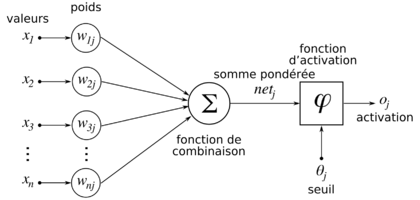
\includegraphics[scale=0.6]{img/neurone.png}}
  \caption{Représentation d'un neurone}
\end{figure}

\noindent Un neurone possède donc une sortie binaire qui découle de la formule suivante :

$$o_{j} = \varphi ((\sum_{i=0}^{n}x_{i} \times w_{i}) - \theta _{j}$$

\noindent La sortie dépend de la fonction et du seuil d'activation qui sont fixés, ainsi que des poids qui composent le neurone. Le réseau de neurones ajuste ces poids durant la phase d'apprentissage afin d'améliorer ses résultats, ce sont donc ces poids que le réseau apprend.\\
 \\
On dit qu'un réseau de neurones est ``profond'' si il est constitué de plusieurs couches de neurones successives (la sortie d'une couche est l'entrée de la suivante): ces réseaux sont souvent plus efficaces sur des problèmes de reconnaissance complexes car les multiples couches leur permettent "d'affiner" successivement ce qui est reconnu (par exemple, pour de la reconnaissance d'images, une première couche pourrait distinguer plusieurs zones de l'image, une seconde les contours des formes qui apparaissent dans ces zones, etc.)

\begin{figure}[h]
  \centerline{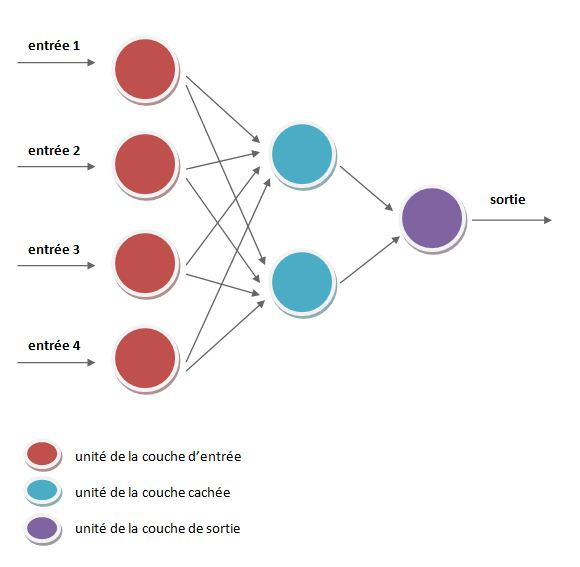
\includegraphics[scale=0.6]{img/organisation_en_couches_rdn.jpg}}
  \caption{Schéma d'un réseau de neurones profond}
\end{figure}

\noindent Le réseau est donc composé de plusieurs couches de neurones qui sont interconnectées.\\  

\subsection{Notre démarche}

L'objectif de ce projet de recherche n'est pas de construire un réseau de neurones par nous-mêmes (nous n'en aurions pas le temps). Pour cette raison, nous allons utiliser une librairie python\footnote{De ce fait, l'intégralité du code que nous allons écrire au cours du projet sera également en python.} qui permet de créer des réseaux de neurones standard de manière très simple et rapide. Notre but sera donc de comprendre comment fonctionne cette librairie, puis de l'utiliser pour construire un (ou plusieurs) réseau qui permettrait de répondre à notre problématique (qui peut donc se résumer par : "Est-il possible d'utiliser un réseau de neurones pour détecter automatiquement la langue d'un contenu audio ?").\\
Les étapes qui suivent résument les différentes parties de notre travail; elles seront détaillées par la suite.\\
 \\
Avant de pouvoir utiliser un réseau de neurones, il est nécessaire de traiter correctement les données dont nous disposons en entrée. Ce prétraitement sera une part importante de notre travail.\\
 \\
\begin{itemize}
  \item Préparation des données (pré-traitement) :
    \begin{dingautolist}{192}
    \item Sélection : Nous avons à disposition un corpus de données audio provenant de sources diverses (émissions de radio, conférences...). Comme tout enregistrement audio, ces fichiers contiennent un certain nombre de passages qui ne sont pas de la parole à proprement dit (musique, applaudissements, silences...), et si ces passages sont trop présents ou trop réguliers, cela risque de biaiser les résultats de notre réseau. Dans un premier temps, nous traiterons donc les fichiers audio afin de supprimer de tels passages.

    \item Paramétrisation : Dans le domaine de la reconnaissance de parole, de manière générale, il est plus efficace de travailler non pas directement avec les signaux audio mais plutôt avec certaines caractéristiques spécifiques extraites de ces signaux. Nous effectuerons donc un traitement acoustique afin d'extraire ces caractéristiques, que l'on mettra en entrée du réseau de neurones.

    \item Stockage : Pour stocker ces ensembles de données, nous utiliserons le format de fichier HDF5, qui permet de classer des groupes de données de manière pratique dans un seul fichier et qui offre certaines options qui nous seront utiles.
    \end{dingautolist}
    
\item Création et utilisation du réseau de neurones
  \begin{dingautolist}{192}
    \addtocounter{enumi}{3}
    \item Formatage des données : Selon son type, un réseau de neurones attend en entrée un ensemble de données organisées de manière spécifique. Nous formaterons donc les données précédemment stockées selon le format d'entrée du réseau utilisé.

    \item Apprentissage et tests : Enfin, il nous restera à créer le réseau proprement dit, puis à réaliser la phase d'apprentissage sur les données formatées. Ensuite , nous pourrons réaliser des tests sur des données nouvelles et affiner les paramètres du réseau pour diminuer son taux d'erreur.
    \end{dingautolist}
  \end{itemize}

\begin{figure}[h]
  \centerline{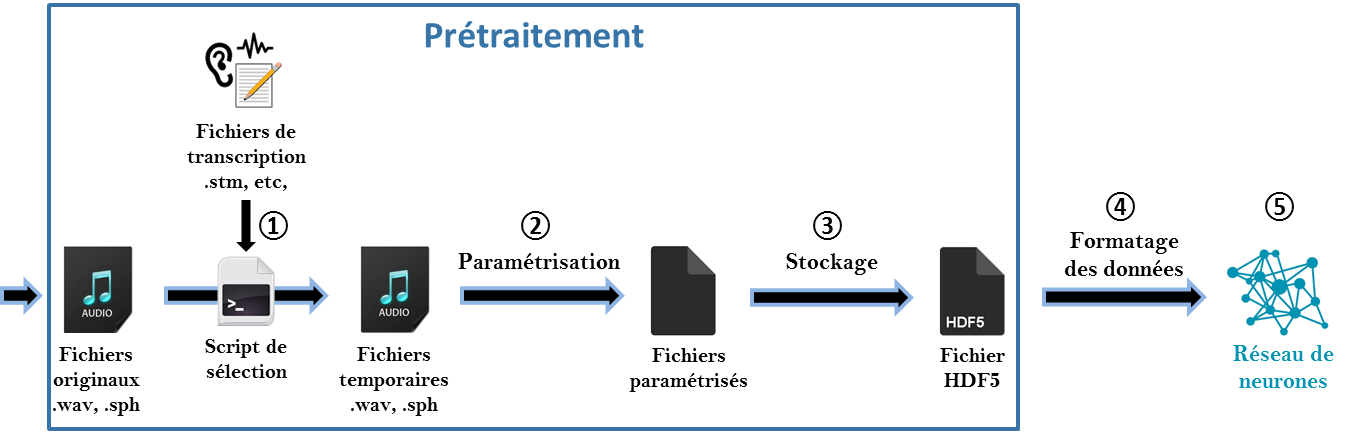
\includegraphics[scale=0.7]{img/schema_complet.png}}
  \caption{Les différentes étapes de notre travail}
\end{figure}
 
\section{Prétraitement : préparation des données}
\hphantom{.}
\begin{figure}[h]
  \centerline{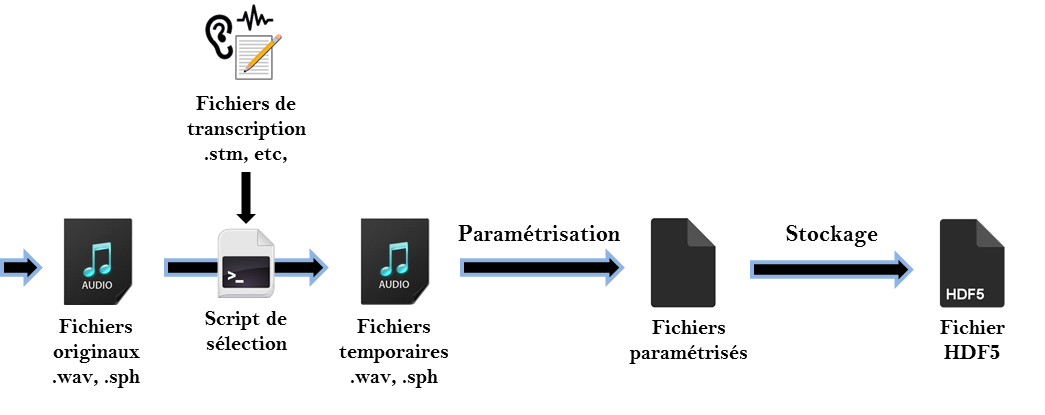
\includegraphics[scale=0.9]{img/schema_pretraitement.png}}
  \caption{Les différentes étapes du prétraitement}
\end{figure}

L'objectif du prétraitement est donc de transformer les données d'entrée (des ensembles de fichiers audio) en un ensemble de données utilisables par le réseau de neurones (des valeurs réelles), stockées sur le disque dur, pour ne pas avoir à refaire le prétraitement à chaque apprentissage du réseau.\\
 \\
 Nous disposons d'un corpus de fichiers de 4 langues différentes (environ une durée totale d'une heure pour chaque) : Arabe, Allemand, Anglais et Français. Les corpus arabe et français sont des extraits d'émissions de radio, le corpus anglais des extraits de conférences, et le corpus allemand des phrases extraites d'un corpus linguistique. En plus des fichiers audio, nous disposons également des fichiers de transcriptions (orthographiques ou phonétiques)\\
*** TRANSCRIPTION ANNEXE ***\\
correspondants qui nous sont utiles pour le prétraitement.

\subsection{Sélection des données utilisables}

\newpage

\hphantom{.}
\begin{figure}[h]
  \centerline{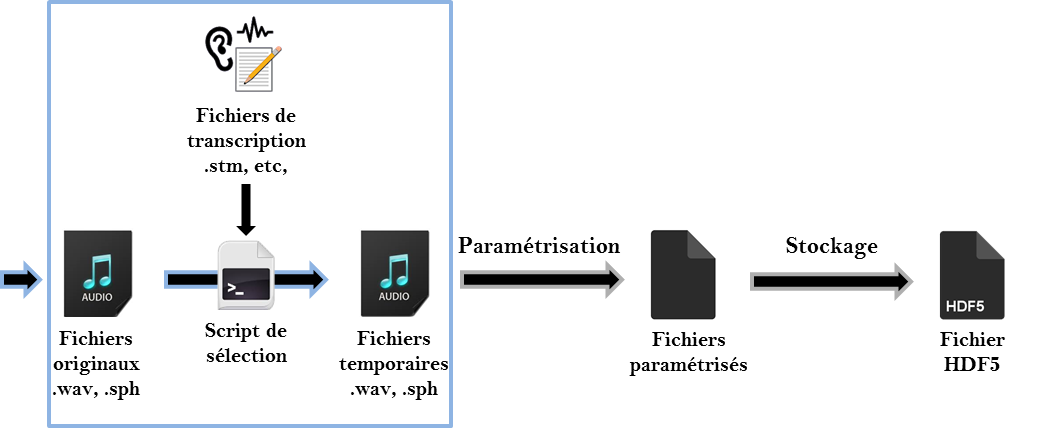
\includegraphics[scale=0.8]{img/schema_selection.png}}
  \caption{La sélection}
\end{figure}

Certains des fichiers audio utilisés peuvent poser problème durant la phase d'apprentissage. En effet, certains commencent ou finissent avec un passage musical ou un silence qui représente une partie non négligeable du fichier. Le problème étant que si un silence ou un passage musical est présent au début ou à la fin dans tous les fichiers audio anglais par exemple, le réseau de neurones risque d'apprendre ce silence ou cette musique comme étant de l'anglais et ainsi de biaiser les résultats sur de futures analyses.\\
\noindent De tels problèmes sont présents sur différents fichiers du corpus dont nous disposons :
\begin{itemize}
    \item les extraits en anglais commencent tous par un morceau musical suivi d'applaudissements ;

    \item les extraits en allemand commencent et se terminent par un silence de durée non négligeable.
    \end{itemize}
    
\noindent Il est donc nécessaire d'enlever ces passages indésirables de manière automatisée. En effet, les retirer à la main aurait demandé beaucoup trop de temps étant donné le grand nombre d'extraits, et il aurait été nécessaire de le refaire pour chaque futur corpus. Pour cela, nous utilisons les transcriptions (orthographiques ou phonétiques) des extraits audio, qui contiennent les temps précis de début et de fin des phrases prononcées.\\
 \\
 Nous avons donc écrit un script afin d'extraire les temps de passage de ``vraie parole'' à l'aide des fichiers de transcription. Pour cela, nous coupons le reste de l'audio des fichiers en utilisant le programme Sox \\
 ***RENVOI VERS SOX***\\(une boîte à outils permettant de faire diverses opérations sur des fichiers audio).

\subsection{Paramétrisation en coefficients acoustiques}

\hphantom{.}
\begin{figure}[h]
  \centerline{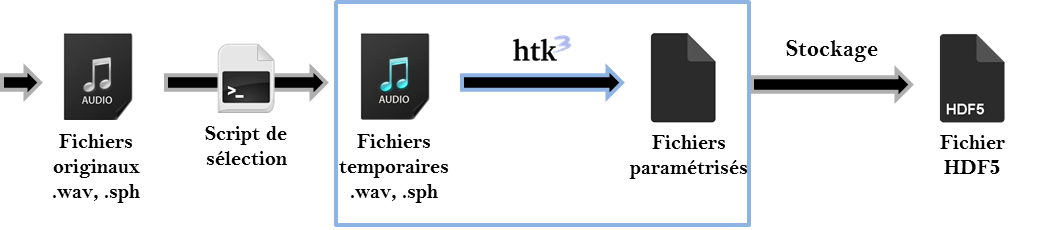
\includegraphics[scale=0.9]{img/schema_parametrisation.png}}
  \caption{La paramétrisation}
\end{figure}
\newpage

Nous pourrions utiliser directement les signaux audio en entrée de notre réseau de neurones : il nous suffirait par exemple de relever la valeur du signal tous les X intervalles de temps et de fournir directement ces valeurs au réseau. Cependant, dans le domaine de la reconnaissance de parole, on utilise plutôt des signaux paramétrisés.
La paramétrisation d'un signal consiste en l'extraction d'un ensemble spécifique de caractéristiques de ce signal. \\
\\
*** A PRECISEEEEEER ***\\
Pour effectuer cette paramétrisation, nous utilisons HTK\\
 ***RENVOI VERS HTK***\\, un logiciel multiplateforme développé par le département d'ingénierie de l'Université de Cambridge, qui est une sorte de ``boîte à outils'' permettant de réaliser toutes sortes de manipulations utiles à la reconnaissance de la parole. Il permet notamment d'effectuer de manière très simple la paramétrisation de fichiers audio en coefficients acoustiques correspondants. Les fichiers ainsi obtenus sont des fichiers .mfcc (Mel-frequency cepstral coefficients).
 
\subsection{Stockage des données}

\hphantom{.}
\begin{figure}[h]
  \centerline{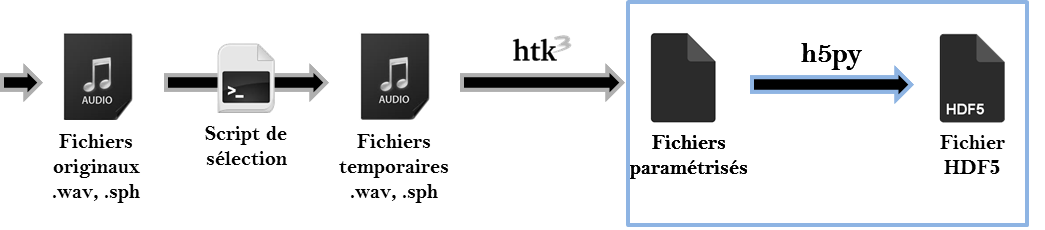
\includegraphics[scale=0.9]{img/schema_stockage.png}}
  \caption{Le stockage des données}
\end{figure}

Afin de ne pas répéter la phase de prétraitement à chaque apprentissage du réseau de neurones, il est primordial de stocker les données pré-traitées. Pour cela, nous utilisons le format de données HDF5\\ ***RENVOI VERS HDF5***\\ (grâce à la bibliothèque python h5py) qui nous permet de hiérarchiser et d'organiser facilement nos données une fois le prétraitement terminé.\\
 \\
 Ce format possède également un autre avantage qui nous est très utile : il permet si nécessaire de transmettre des données en les chargeant directement depuis le disque dur. En effet, pour éviter les régularités dans les fichiers de données qui pourraient biaiser le processus d'apprentissage, les données en entrée du réseau de neurones seront mélangées avant le début de l'apprentissage. Pour ce faire, il est nécessaire de lui fournir l'intégralité des données en une seule fois. De ce fait, la quantité de données générée par la transformation des fichiers audio en coefficients acoustiques peut être trop importante pour pouvoir charger les données directement en mémoire vive selon la taille de départ du corpus. Le format de données HDF5 nous permet donc de parer à ce problème éventuel en chargeant les données directement depuis le disque dur sans surcharger la mémoire vive, même si la vitesse de traitement s'en trouve diminuée.\\
 \\
Au final, la taille des données ne nous a pas posé de problème, étant suffisamment petite pour être chargée en mémoire. Néanmoins, nous avons quand même écrit une fonction qui utilise cette caractéristique du format HDF5, qui pourrait être utile dans le futur, si on a un jour besoin de traiter plus de données.

\section{Utilisation des réseaux de neurones}

\hphantom{.}
\begin{figure}[h]
  \centerline{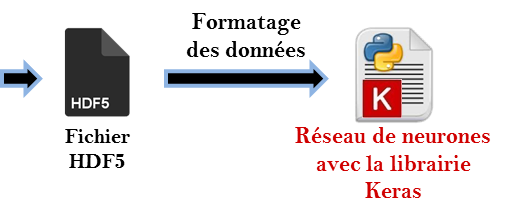
\includegraphics[scale=0.9]{img/schema_reseau_keras.png}}
  \caption{L'utilisation du réseau de neurones}
\end{figure}

Une fois les données mises en bonne forme dans notre fichier HDF5, nous pouvons les transmettre au réseau de neurones et de commencer l'apprentissage. Pour cela, il nous faudra formater les données sous la forme attendue par le réseau (qui pourra changer selon le type de réseau construit) et trouver les bons paramètres pour le réseau qui nous permettront d'obtenir de meilleurs taux de reconnaissance.

\subsection{Keras}

Keras est une librairie open-source Python utilisée pour construire, entraîner et manipuler des réseaux de neurones artificiels, développée par François Chollet dans le cadre du projet de recherche ONEIROS (Open-ended Neuro-Electronic Intelligent Robot Operating System). L'avantage de cette librairie est qu'elle est très haut niveau, elle permet donc de créer des réseaux de neurones très rapidement et très simplement. En effet, cette dernière n'est en quelque sorte qu'une "interface de surcouche" qui se place au-dessus de librairies de réseaux de neurones plus bas niveau comme Theano, qui est la sous-couche que nous utiliserons avec Keras.\\
 \\
Il est possible de créer un réseau de neurones (parfois complexe) avec Keras en littéralement quelques lignes :

\lstlisting{model = Sequential()            # création d’un modèle séquentiel
model.add(Dense(units=64, input_dim=100))    # ajout d’une couche
model.add(Activation('relu'))            # et de sa fonction d’activation

model.compile(loss='categorical_crossentropy', optimizer='sgd', metrics=['accuracy'])            # permet de configurer différents paramètres de la phase d’apprentissage du réseau

# lance la phase d’apprentissage sur 5 epochs
model.fit(x_train, y_train, epochs=5, batch_size=32)}

De plus, Keras est très pratique à utiliser en python (les réseaux créés fonctionnant avec des tableaux numpy classiques\footnote{Numpy est une bibliothèque scientifique très utilisée en Python, qui offre notamment la possibilité de réaliser simplement des calculs matriciels.}) et dispose de beaucoup d'options, qui permettent par exemple d'interrompre l'apprentissage dès qu'on le juge nécessaire, de sauvegarder un modèle de réseau, d'optimiser la lecture depuis un fichier HDF5...

\subsection{Définir l'architecture du réseau}

\subsection{Apprendre les paramètres du réseau sur le corpus d'apprentissage}

\subsection{Utiliser le réseau pour étiqueter le corpus de test}



\section{Conclusion}

\bibliographystyle{plain}
\bibliography{biblio}

\end{document}
